\documentclass[a4paper,twocolumn,10pt]{article}
\usepackage[margin=1in]{geometry}
\usepackage{listings}
\usepackage[utf8]{inputenc} % allow utf-8 input
\usepackage[T1]{fontenc}    % use 8-bit T1 fonts
\usepackage{hyperref}       % hyperlinks
\usepackage{url}            % simple URL typesetting
\usepackage{booktabs}       % professional-quality tables
\usepackage{amsfonts}       % blackboard math symbols
\usepackage{nicefrac}       % compact symbols for 1/2, etc.
\usepackage{microtype}      % microtypography
\usepackage{lipsum}     % Can be removed after putting your text content
\usepackage{graphicx}
\usepackage{titlesec}
\usepackage{fancyhdr}
\usepackage{siunitx}
\usepackage{amsmath}
\usepackage{CJKutf8}
\usepackage{float}
% \renewcommand{\thempfootnote}{\arabic{footnote}}
\makeatletter
\newcommand\footnoteref[1]{\protected@xdef\@thefnmark{\ref{#1}}\@footnotemark}
\makeatother
\pagestyle{fancy}
\titleformat{\section}{\large\scshape}{\thesection}{1em}{}
\titleformat{\subsection}
  {\normalfont\scshape}{\thesubsection}{1em}{}
\titleformat{\subsubsection}
  {\normalfont\scshape}{\thesubsubsection}{1em}{}
\pagenumbering{arabic}
\newtheorem{definition}{Definition}[section]
\usepackage[backend=biber,style=ieee,natbib=true]{biblatex}
\renewcommand{\bibfont}{\footnotesize} % for IEEE bibfont size
\addbibresource{citations.bib} %added

\usepackage{csquotes}

\title{\vspace{-50pt}\bfseries{\Large{Midi Shark: For Piano Transcription}}}
\author{\normalfont{Jonah Chen, QiLin Xue, Joe Hattori, Khanatat Thangwatthanarat}\\\small{University of Toronto}\\\vspace{-10pt}\small{\url{{jonah.chen,qilin.xue,joe.hattori,k.thangwatthanarat}@mail.utoronto.ca}}}
\date{\today}
\begin{document}
\maketitle
\section{Introduction}
Transcription of music is the process of determining the pitches and timing of notes from recorded audio files. Transcription has always been a specialized task that requires years of musical training. Transcription is even more challenging for polyphonic music, such as piano, which features the simultaneous production of two or more tones. The majority of traditional transcription models focus on extracting all of the notes from the recording using the node onset. This, however, is not the way a trained musician approaches the problem\cite{intro}.

We developed a model that is more accurate at transcribing piano recordings by analyzing the recording with a neural network and focusing on both the onsets and offsets of the node. Moreover, since images and audios both have common two-dimensional time-frequency input representations, the fact that CNN performs well in image classification problems suggests that CNN could potentially be used for music transcription\cite{onsets_and_frames}.

\section{Illustration}
The model architecture is shown in figure \ref{fig:architecture}.
\begin{figure}[h!]
  \centering
  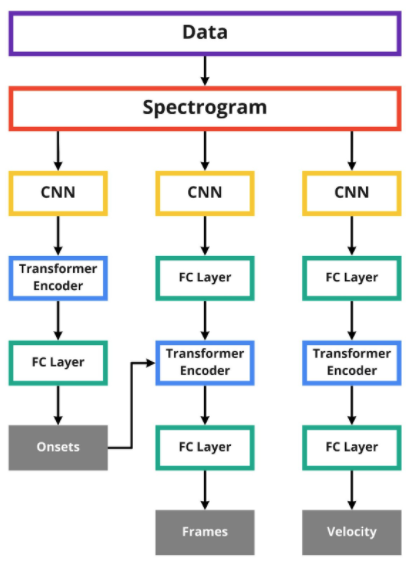
\includegraphics[width=0.7\linewidth]{figures/architecture.png}
  \caption{Model architecture}
  \label{fig:architecture}
\end{figure}

\section{Background}
Polyphonic automatic music transcription is a difficult task due to the potential of having multiple notes played simultaneously, causing the harmonics of each note to overlap with the others. Therefore, it is a non-trivial task to transcribe the music using the spectrogram. 

Since the advent of machine learning, there have been models developed for solving this problem. A relatively successful model is the Onsets and Frames (OF) model developed by the Google Brain Team using TensorFlow in 2017 and implemented into the open-source “magenta” framework[9]. This model uses a two-headed encoder-decoder architecture that predicts onsets (when the notes are played), and frames (what notes are played at the onset). This model uses convolutional neural networks as encoders and bidirectional LSTM as decoders and was able to achieve an F1 score of 78.30\% and 82.29\% on frames and notes respectively for the MASTERO dataset, which is arguably the largest dataset for music transcription task.

\section{Data Processing}
The Maestro dataset consists of pairs of WAV and MIDI files of piano audio separated by year. The years consists of $2004,2006,2008-2018.$ The audio in $2017$ served as the validation set and the audio in $2018$ served as the test set. In total, there are over $200$ hours of piano performances.

To process the WAV files to act as inputs, we converted them to frequency spectrograms by applying a Short-Time Fourier Transform using a sampling rate of $16000$, and used the Mel scale for the frequency in order to generate $229$ bands. Since songs can be up to $30$ minutes, and transformers have a time complexity of $\mathcal{O}(n^2),$ we are motivated to keep sequence lengths short. As a result, we partitioned the spectrogram into $20s$ non-overlapping segments such that each segment has a shape of $229 \times 862.$

The MIDI files acted as the ground truth, but the files only contained information about the onset and offset of each note. We preprocessed each midi file into three arrays of shape $88 \times 862,$ where $88$ is the number of notes. Each entry $(t,n)$ denotes the value of the array at a specific time $t$ and a note $n$.
\begin{itemize}
  \item Onset Array: We have $(t,n)=1$ if the note $n$ is played at time $t$ but not played at time $t-1.$
  \item Frames Array: We have $(t,n)=1$ if the note $n$ is played at time $t$.
  \item Velocities Array: We have $(t,n)=v/127$ where $v \in [0,127]$ is the velocity of the note, which is an indicator of the dynamics.
\end{itemize}
These arrays act as the labels for each of the three sub-tasks described in figure \ref{fig:architecture}.
Our data processing can be broken down to two major parts. One is converting WAV files to spectrograms, and the other task is converting MIDI files to a certain kind of form which is easier to train the model.

We chose to convert MIDI files into arrays with time on the x-axis and note on the y-axis. As MIDI files hold when each note begins, how long it lasts, and how strong it was played, we divided MIDI files into three arrays respectively; first array is onsets array, the second array is frames array, and the third array is velocity array.

Since every song has a different length, we divided all the spectrograms and the labels into 20 second segments, so our model will take a 20 second long spectrogram as input.

The downside of this approach is that we might have a clip at the end of the song that is shorter than 20 seconds. This can be resolved by zero-padding, however, since most songs were several minutes long, we did not think this would make a noticeable difference and opted to simply ignore these last few seconds.
\section{Architecture}
The OF model\cite{onsets_and_frames} had seen success in the task of automatic music transcription, but since 2017 when the model was published, there have been several publications that have brought forth improvements in areas like sequence processing.

In the OF model, the processed mel-spectrogram data is encoded using a stack of convolutional layers\cite{rainer}. Furthermore, the OF model uses bidirectional LSTM models as decoders. Since 2017, the transformer architecture has revolutionized the processing of sequential data\cite{attention}. Many of today’s state-of-the-art models in fields like natural language processing are based on the transformer. As audio is sequential data, we think it will be advantageous to use a transformer encoder in place of the bidirectional LSTM.

Following similar data flow to OF, we will have a two-headed model with an onset and frame head. The onset prediction is passed as an input to the transformer encoder that decodes the frame predictions. We use the same loss functions for the two heads from OF (a generalization of cross-entropy loss, see eq.1-6 in\cite{onsets_and_frames}). For the velocity model, we use a similar approach to the frames model but without the input from onset prediction. Apart from that, we use the modified version of mean square error instead of a cross-entropy loss as a loss function. For all the models, we use Adam optimizer as our optimization function.  For all the models, we also use fully connected layers in between. For a clearer picture of the model structure, please refer to figure 1 in the introduction section.

\section{Baseline Model}
The baseline model we compare our model to is the LSTM described in the \textit{Onsets and Frames} paper by Google\cite{onsets_and_frames}. The model architecture is very simlar to figure \ref{fig:architecture}, except transformers are used instead of LSTMs, and the onsets do not feed back into the LSTM.

This is a reasonable choice since our hypothesis is that introducing a transformer will improve the performance of the model. Since Google researchers likely have far greater computing resources than us and better data processing, to create a better comparison, we will write and train the LSTM model on the same processed data and machine used for the Transformer model.  



\section{Quantitative Results}

A piano has 88 keys but a human only has 10 fingers. On average, less than $5\%$ of the notes are pressed at any given time. If we were to use accuracy as our metric, a model that predicts no notes at all would achieve over $95\%$ accuracy. Clearly, accuracy is not a good indicator of the performance of a model. Instead, we opted to use the F1 score
\begin{equation}
  F1 = \frac{2PR}{P+R}
\end{equation}
where $P$ is the precision, $R$ is the recall. We used the test split of the MAESTRO dataset which was never used in training or hyperparameter tuning.

\begin{table}[H]
  \begin{minipage}{\linewidth}
    \centering
    \begin{tabular}{|c|c|}
        \hline
        Model& Frames F1 Score \\
        \hline
        Sigtia et al., 2016 & \(72.22\%\)\\
        \hline
        Kelz et al., 2016 & \(71.60\%\)\\
        \hline
        Melodyne\footnote{Commercial software, not machine learning model.} & \(58.57\%\)\\
        \hline
        OF & \(78.30\%\)\\
        \hline
        \textbf{Google’s 2021 Model} & \(\mathbf{82.18\%}\)\\
        \hline
        Baseline Model (LSTM)\footnote{Same architecture as OF, but trained by us with the same hyperparameters.}\footnoteref{fn:midishark} & \(74.44\%\)\\
        \hline
        Midi Shark (Us)\footnote{\label{fn:midishark}Tested on the test split of the MAESTRO dataset, because the MAPS dataset is unavailiable due to website failure.} & \(79.01\%\)\\
        \hline
    \end{tabular}
  \end{minipage}
\end{table}

For the velocity model, we used a different metric. As the velocities represent the intensity of the notes we hear, we track the number of notes (onsets) that are predicted to be played, which are within \(\{10\%, 3\%, 1\%\}\) of the ground truth velocities. Our velocity model achieves \(\{95.78\%, 59.46\%, 21.48\%\}\) on these metrics respectively. The baseline model achieves ..., again indicating the transformer encoder was able to outperform the LSTM.

\section{Testing}
One concern is that the music in the Maestro dataset share similar features. They are mostly classical pieces from the 17th to early 20th century\cite{maestro}, and there could be inherent biases the creators of the dataset might have when selecting the pieces and the type of recording device used.

We decided to record our own music. In the spirit of having a much different style than the music in the dataset, we recorded an \textit{anime} song played in \begin{CJK}{UTF8}{min}なんでもないや.\end{CJK}

Since we don't have the ground truth, and there were some mistakes made while playing it, we decided to use a holistic evaluation instead, which is what matters at the very end. The generated audio is linked in the Github repository.

In general, the generated audio sounds very good and captures the main melody, harmony, and dynamics. However, it fails to capture some lower notes. This makes sense as it is difficult to pick up lower frequencies through a microphone, and the microphones the Maestro dataset used to record was likely calibrated to better capture the lower frequencies.

Furthermore, there are a few false positives that is exactly one octave above the melody. This also makes sense because it corresponds to the first overtone of the melody, which also happens to be the most dominant one. These same characteristics was found when testing the model on other music found on Youtube, though the quality heavily depended on the quality of the recording device.

To fix this in future models, we can augment our training data by adding in random noise that is consistent with poor microphone quality. This will allow the model to perform better on new data that is not recorded with a professionally calibrated microphone.
\section{Discussion}
\section{Ethical Considerations}
In the United States, the music sheet industry is worth around 1 billion USD\cite{musicspoke}. A technology that can transcribe music may render purchasing music sheets useless. Many of these sales come from music books, which often contain several scores that can be readily found online, so big publishers will likely not be greatly affected by this technology.

However, this technology will negatively affect small composers, who may make a living by selling sheet music to their music, for example on services such as MusicSpoke\cite{musicspoke}. If this technology is accurate and readily available, it may encourage musicians to automatically generate the sheet music to the songs they like, instead of purchasing and supporting artists. Fortunately, transcribing isn’t just about having the right notes, but the style in which it is presented. This is why two transcribers will not produce the same sheet music for the same song.

The MASTERO dataset and the scope of our project consist of working solely with music, so there is a low risk of discriminating against humans from pre-processing to training and post-processing. However, a large majority of the music from the dataset is Western music, so the results would likely be more reliable towards Western music. Thus, people from other cultures may not find the same success in this model as people in Western cultures do. To address this, we will attempt to find other similar datasets that were trained on music from other cultures.
\printbibliography
\end{document}